\section{Implementering}
Implementering af systemets funktionalitet tager udgangspunkt i de udarbejdede hardware- og softwarediagrammer. Hardwarediagrammer bruges til at definere hvordan systemets hardware kobles, mens softwarediagrammerne bruges til at definere og implementere software.

Implementeringsfasen udarbejdes iterativt, og de højst prioriterede use cases implementeres først. 
Dette afsnit beskriver implementering af systemet.

\subsection{Drone}
Drone indeholder alt systemets hardware. Software til drone er udviklet i programmerings sproget C++, og er opdelt i forskellige ansvarsområder. Nogle softwareklasser bruges til at aflæse data fra højdesensor, 3G/GPS modul og kompas, mens andre klasser er ansvarlige for kommunikation. Information fra de forskellige softwareklasser samles og behandles på dronens main controller. Ud fra den indsamlede data tilpasses dronens flyveindstilling via dertil indrettede klasser. 

Håndtering af GPS sker via den abstrakte \textit{GPS} klasse og \textit{StandAloneGps} klassen der nedarver fra den abstrakte klasse. Når nuværende og ønsket GPS position kendes, kan korrekt flyveretning og afstand til ønsket GPS position findes. Til at finde korrekt flyveretning og afstand til ønsket GPS bruges de to metoder \textit{calBearingToTarget} og \textit{calDistToTarget} fra \textit{FlightControl} klassen. 

Dronen kommunikerer med server via HTTP protokollen, til dette anvendes flere klasser. GetAndPut klassen som er den mest hardware nære klasse, håndterer \textit{GET} og \textit{PUT} requests. Metoder i \textit{GetAndPut} klassen anvendes af de to klasser, \textit{EventHandler} og \textit{WayPointsHandler}. Disse klasser sorterer informationen fra \textit{GetAndPut} og returnerer det nødvendige information. \textit{Communication} klassen bruger Handler klasserne, hvilket giver systemet lav kobling. Ved at have denne opdeling, er klasserne uafhængige af hinanden og tests kan udføres enkelt.

Under flyvning aflæser main controller løbende flyvehøjde fra ultralydssensor via \textit{DistanceSensor} klassen og nuværende orientering fra flight control boardet via \textit{FlightControl} klassen. \textit{FlightControl} klassen benyttes også når der på baggrund af indsamlet data er brug for ændring af flyveindstilling, eksempelvis korrektion af \textit{throttle}. I \textit{FlightControl} klassen er der dels implementeret metoder, der initierer timere som kontrollerer PWM styrings signaler. Desuden er der implementeret set-metoder der anvendes til korrektion af \textit{throttle}, \textit{yaw}, \textit{picth} og \textit{roll}.  

Af sikkerhedshensyn er det implementeret, at bruger med en fjernbetjening kan skifte fra autonom til manuel styring. Under flyvning kalder main controller løbende metoden \textit{checkIfControllerIsOn}, for at kontrollere hvorvidt dronen skal styres autonomt eller manuelt.  

\subsection{Server}
Indledningsvis i implementeringen blev der lagt meget fokus på server, da den spiller en afgørende rolle i kommunikationen mellen drone og webapplikation. 
Server er udviklet i programmerings sproget Python og med webframeworket Django[x].
Tilsammen udgør Python og Django en SQLite database med et RESTful API. Der benyttes en række API-endpoints for at tilgå eller ændre data på server.

Databasen er designet modulært så systemet har stor mulighed for udvidelser, fx. mulighed for at håndtering flere brugere og flere droner. Omdrejnings punktet i databasen er et event, der indeholder information omkring hvilke bruger som har oprettet event og til hvilke droner.

Til udviklingen af serveren er der også benyttet Django REST frameworket[x], som er en udvidelse til Django. Ved brug af dette framework kan tags som "@api\_view(['GET', 'POST'])" benyttes til at fortælle server hvilke HTTP requests der er tilladt til et givet endpoint. 
Ved brug af REST frameworket kan der gøres brug af serializers, som bruges til at informere  serveren om hvordan data skal formateres på. Med et browsable API simplificeres udviklingen med frameworket.

\newpage
\subsection{Webapplikation}
Webapplikationen  er udviklet i programmeringssprogene HTML, CSS og JavaScript. Webapplikationens frontend er udviklet med frameworket AngularJS[X], som er et meget vidt benyttet framework udviklet af Google. Derudover benyttes et google maps API til webapplikationen. Dette API muliggør brugen af kort på webapplikationen. Da AngularJS er benyttet til udviklingen, er projektet opdelt efter MVC-modellen[x]. 

Kortet er implementeret ved brug af et google-maps directive[X], dette pakker google maps api'et ind og derved gør det mere effektivt i forbindelse med Angular udvikling. Dette betyder også at noget funktionalitet som google maps tilbyder kan ikke direkte bruges i dette directive. 
Da det var et krav at waypoints skulle oprettes ved klik på kortet, blev der udviklet et specifik klik event på kortet. Når et klik på kortet finder sted bliver der tegnet et waypoint på kortet. I koden bag bliver der så oprettet to waypoint objekter. Det ene waypoint objekt er til kortet, dette objekt indeholder kun icon, latitude og longitude til hvor waypointet skal tegnes. Det andet waypoint, der bliver oprettet, er det waypoint som skal benyttes og sendes til serveren når brugeren ønsker at publicere det tegnede rute. Dette er nødsaget da google-maps directivet ikke kan finde ud af at tegne waypoints hvis de indeholder data som directivet ikke kender til. Figur \ref{fig:click_event} illustrere hvordan klik eventet opretter to waypoint objekter.

\vspace{-5pt}
%kommentar
\begin{figure}[H]
	\centering
	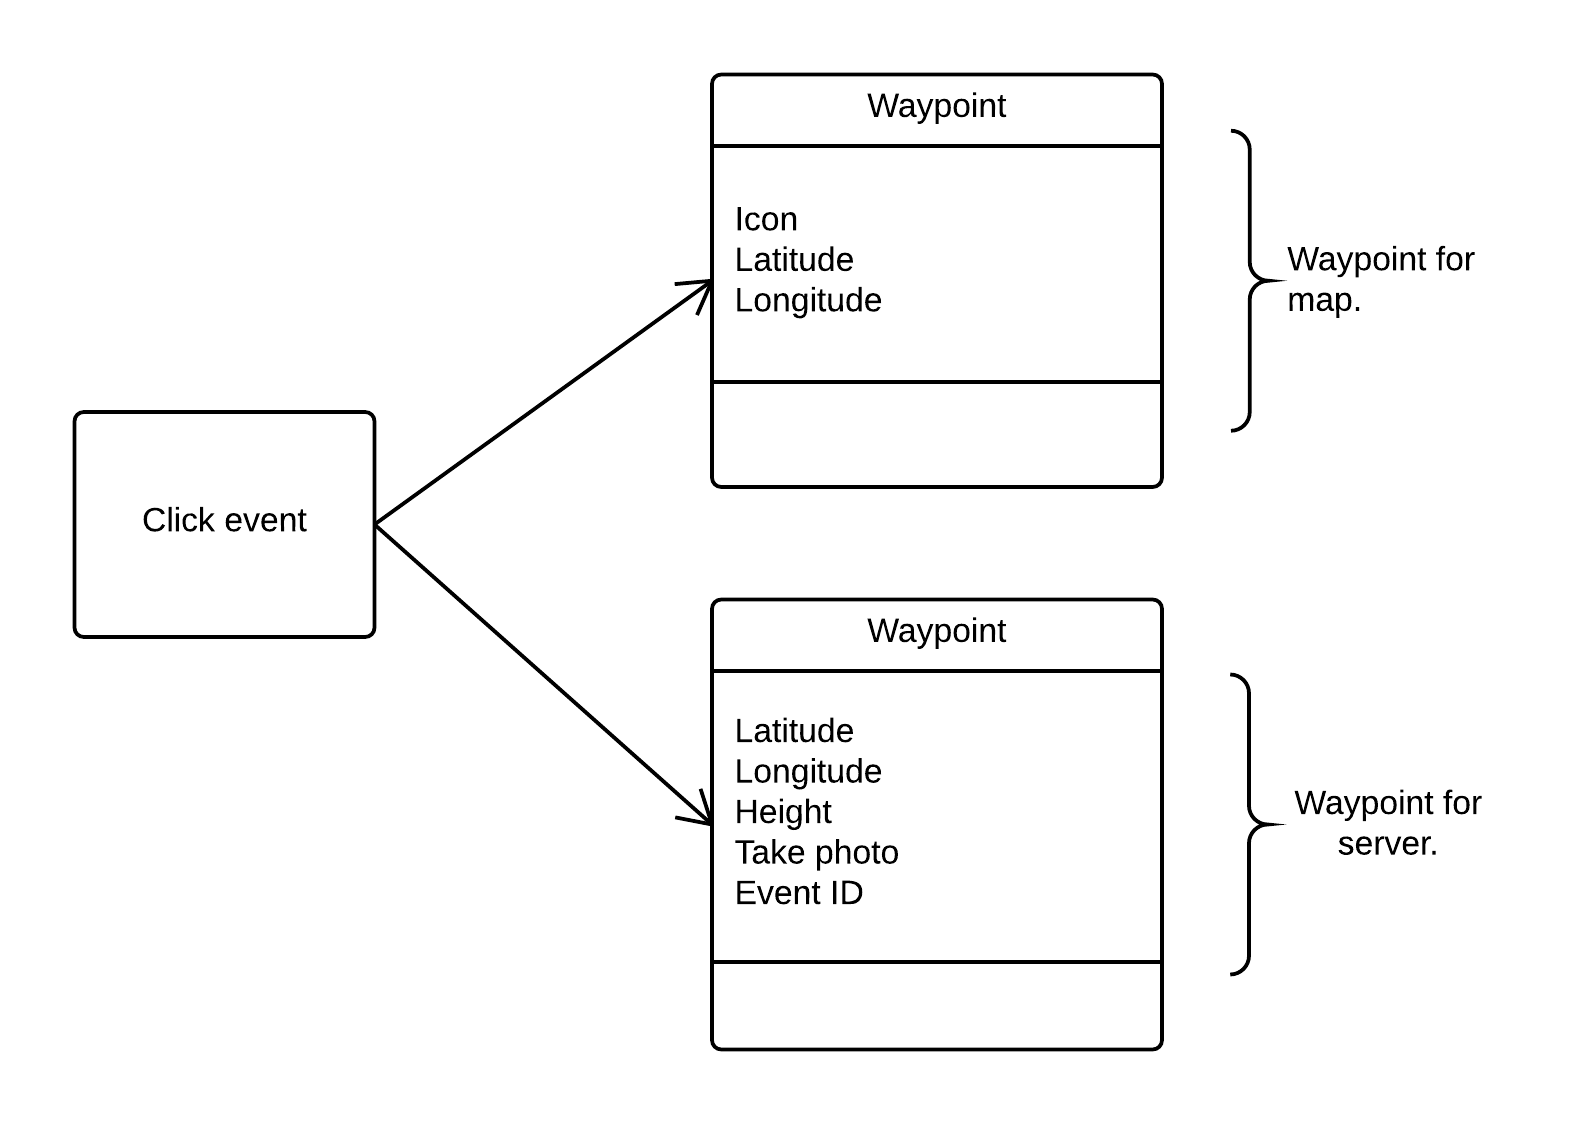
\includegraphics[width=0.6\textwidth]{Billeder/click_event.png}
	\vspace{-5pt}
	\caption{Click event eksempel}
	\label{fig:click_event}
\end{figure}


Under udviklingen af webapplikationen har test vægtet en stor del, systemet skulle udvikles, så det var testbart. Derfor blev der brugt AngularJS's dependency injection teknikker. Alt kommunikationen med backend'en er for et eksempel skrevet som en service, som alle andre services og controller benytter sig af via dependency injection, på den måde kan alt kommunikation til serveren abstraheres væk. Lignende teknikker er benyttet for alle services i systemet, som indeholder størstedelen af logikken i systemet.  

Alle requests til server sker asynkron. Derfor er webapplikationen implementeret således at når der bliver lavet et request til server, så arbejder webapplikationen videre og når data fra serveren er klar så får webapplikationen et interrupt og præsentere data. Dette kan ses ved klik på kortet, hvor efter et kort delay dronen bliver tegnet på kortet.

